\documentclass{beamer}
% \usepackage{beamerthemesplit}
\usetheme{Madrid}
% \usepackage{pstricks}
\usepackage{graphicx}
\usepackage{mdwlist}
\usepackage{lineno, hyperref}
\usepackage{stackrel}
\usepackage{changepage}

\usepackage{amssymb,latexsym,amsmath,amsthm,bbm}
\usepackage{hyperref}
\usepackage{tikz}
\usepackage[english]{babel}
\usepackage[latin1]{inputenc}
\usepackage[authoryear]{natbib}
\usepackage{multirow}
\usepackage{verbatim}
\usepackage{alltt}
\usepackage{mycommands}

% \usepackage{cmbright}
\renewcommand*\familydefault{\sfdefault}
\usepackage[T1]{fontenc}


\definecolor{wp-red}{RGB}{204,0,0}
\definecolor{wp-gray}{RGB}{51,51,51}
\definecolor{reynolds-red}{RGB}{153,0,0}
\definecolor{pyroman-flame}{RGB}{209,81,34}
\definecolor{hunt-yellow}{RGB}{253,215,38}
\definecolor{genomic-green}{RGB}{125,140,31}
\definecolor{innovation-blue}{RGB}{66,126,147}
\definecolor{bio-indigo}{RGB}{65,86,161}

\setbeamercolor{structure}{fg=wp-red}
\setbeamercolor{title}{bg=white, fg=wp-red}  % changes color on title page
\setbeamerfont{title}{series=\bfseries, size=\huge}
\setbeamerfont{author}{series=\bfseries, size=\large}
\setbeamerfont{institute}{series=\mdseries, size=\large}

\setbeamercolor{frametitle}{bg=wp-red, fg=white}  % changes color at top of frame
\setbeamerfont{frametitle}{series=\bfseries}
\setbeamercolor{title in head/foot}{fg=white, bg=wp-red}  % changes color for title in footer
\setbeamerfont{title in head/foot}{series=\bfseries}
\setbeamercolor{author in head/foot}{fg=white,bg=wp-gray}  % changes color for author in footer
\setbeamerfont{author in head/foot}{series=\bfseries}

\newcommand{\btheta}{ \mbox{\boldmath $\theta$}}
\newcommand{\blambda}{ \mbox{\boldmath $\lambda$}}
\newcommand{\bmu}{ \mbox{\boldmath $\mu$}}
\newcommand{\bsigma}{ \mbox{\boldmath $\sigma$}}
\newcommand{\balpha}{ \mbox{\boldmath $\alpha$}}
\newcommand{\bbeta}{ \mbox{\boldmath $\beta$}}
\newcommand{\bdelta}{ \mbox{\boldmath $\delta$}}
\newcommand{\bgamma}{ \mbox{\boldmath $\gamma$}}
\newcommand{\brho}{ \mbox{\boldmath $\rho$}}
\newcommand{\bnu}{ \mbox{\boldmath $\nu$}}
\newcommand{\bpsi}{ \mbox{\boldmath $\psi$}}
\newcommand{\btau}{ \mbox{\boldmath $\tau$}}
\newcommand{\bepsilon}{ \mbox{\boldmath $\epsilon$}}
\newcommand{\beps}{ \mbox{\boldmath $\varepsilon$}}
\newcommand{\bX}{ \mbox{\boldmath X}}
\newcommand{\bx}{ {\bf x} }
\newcommand{\by}{ \mbox{\boldmath y}}
\newcommand{\bY}{ \mbox{\boldmath Y}}
\newcommand{\bz}{ \mbox{\boldmath z}}
\newcommand{\bZ}{ \mbox{\boldmath Z}}
\newcommand{\bW}{ \mbox{\boldmath W}}
\newcommand{\bb}{ \mbox{\boldmath b}}
\newcommand{\bg}{ \mbox{\boldmath g}}
\newcommand{\bL}{ \mbox{\boldmath L}}
\renewcommand{\bs}{ \mbox{\boldmath s}}
\newcommand{\bt}{ \mbox{\boldmath t}}
\newcommand{\bu}{ \mbox{\boldmath u}}
\newcommand{\bv}{ \mbox{\boldmath v}}
\newcommand{\ba}{ \mbox{\boldmath a}}
\newcommand{\bfe}{ \mbox{\boldmath e}}
\newcommand{\bE}{ \mbox{\boldmath E}}
\newcommand{\bV}{ \mbox{\boldmath V}}
\newcommand{\bM}{ \mbox{\boldmath M}}
\newcommand{\bA}{ \mbox{\boldmath A}}
\newcommand{\skewt}{skew-$t$ }
\newcommand{\Skewt}{Skew-$t$ }

\newcommand{\STGP}{ \cal{STGP}}
\newcommand{\GP}{ \cal{GP}}

% \newcommand{\argmin}{{\mathop{\rm arg\, min}}}
% \newcommand{\argmax}{{\mathop{\rm arg\, max}}}
% \newcommand{\iid}{\stackrel{iid}{\sim}}
\newcommand{\bit}{\begin{itemize}}
  \newcommand{\eit}{\end{itemize}}

% \newcommand*\oldmacro{}
% \let\oldmacro\insertshorttitle
% \renewcommand*\insertshorttitle{
%   \oldmacro\hfill
%   \insertframenumber\,/\,\inserttotalframenumber}

\title[\Skewt model for threshold exceedances]{A Space-time \skewt model for threshold exceedances}
\author[S. Morris]{Samuel A. Morris}
\institute[]{North Carolina State University}
\date[]{August 3, 2016}

% \subject{Talks}

%%% NCSU BLOCK %%
% \pgfdeclareimage[height=1.6cm]{ncsu-block}{ncsu-block}
% \logo{\pgfuseimage{ncsu-block}}

%%% NCSU LOGO %%
% \pgfdeclareimage[height=1.5cm]{75year}{75year}
% \logo{\vspace{195px}\pgfuseimage{75year}}

% \AtBeginSection[]
% {
%   \begin{frame}<beamer>
%   \frametitle{Outline}
%   \tableofcontents[currentsection,currentsubsection]
%   \end{frame}
% }

% \AtBeginSubsection[]
% {
%   \begin{frame}<beamer>
%   \frametitle{Outline}
%   \tableofcontents[currentsection,currentsubsection]
%   \end{frame}
% }

% If you wish to uncover everything in a step-wise fashion, uncomment
% the following command:

%\beamerdefaultoverlayspecification{<+->}
% \newcommand{\Href}[2]{\href{#1}{\textcolor{blue}{#2}}}

\begin{document}

\begin{frame}
  \titlepage


\begin{center}
   Joint work with Brian Reich (NCSU), Emeric Thibaud (CSU), and Dan Cooley (CSU)
\end{center}
\end{frame}


% \begin{frame}\frametitle{I reached my 5-year return level!}
%   \begin{center}
%     \includegraphics[height=0.7\textheight]{Pic/tunnel_mountain}
%   \end{center}
%  Thanks to the organizers. The meeting has be great.
% \end{frame}


% \begin{frame}\frametitle{Sam Morris}
%   \begin{center}
%     \includegraphics[height=0.7\textheight]{Pic/Sam}
%   \end{center}
% \end{frame}


\begin{frame}\frametitle{Spatial extremes}
 \bit\setlength\itemsep{\fill}
  \item Extreme Values Analysis (EVA) can benefit greatly from spatial methods
  \item Spatial methods can map risk and borrow strength over space to estimate rare-event probabilities
  \item Accounting for spatial dependence is necessary for valid inference
  \item Methods and software in this area are developing rapidly to meet a growing demand
 \eit
\end{frame}

\begin{frame}\frametitle{Max-stable processes}
  \bit\setlength\itemsep{\fill}
  \item Let $Y_1(\bs)$, ..., $Y_m(\bs)$ be iid spatial processes
  \item The pointwise maximum process is $${\tilde Y}(\bs) =\bigvee_{l=1}^m Y_l(\bs)$$
  \item If there exist constants $a_m$ and $b_m$ so that $$Z(\bs)= a_m + b_m {\tilde Y}(\bs)$$
  converges to a valid process as $m\rightarrow\infty$, then $Z$ is max-stable
  \eit
\end{frame}

\begin{frame}\frametitle{Max-stable processes}
  \bit\setlength\itemsep{\fill}
  \item The marginal distribution of $Z$ at each $\bs$ follows generalized extreme value (GEV) distribution
  \item Distribution function is $F(z) = \exp\{-t(z)\}$ where
  \begin{align*}
      t(z) = \left\{ \begin{array}{ll}
        \left[1 + \xi \displaystyle \left(\frac{z - \mu}{\sigma}\right)\right]^{-1 / \xi}, \quad &\xi \neq 0 \\ [1em]
        \exp\left\{- \displaystyle \frac{z - \mu}{\sigma}\right\}, &\xi = 0.
    \end{array}\right.
  \end{align*}
  % \item Three parameters:
  % \begin{itemize}
    \item Location: $\mu \in \mathcal{R}$
    \item Scale: $\sigma > 0$
    \item Shape: $\xi \in \mathcal{R}$
  % \end{itemize}
  \eit
\end{frame}

\begin{frame}\frametitle{Challenges in EVA}
  \bit\setlength\itemsep{\fill}
  \item Covariance focuses on deviations around the mean and not the extremes
  \item Want dependence measure to capture likelihood of seeing values that are jointly extreme
  \item Two common measures of dependence: \vspace{0.5em}
  \begin{itemize}
    \item Extremal coefficient $\vartheta \in (1, 2)$: $$\mbox{Prob}[Z(\bs_1)<c, Z(\bs_2)<c] = \mbox{Prob}[Z(\bs_1)<c]^{\vartheta(\bs_1,\bs_2)}$$
    \item $\chi \in (0, 1)$: $$\chi(\bs_1,\bs_2) = \lim_{c\rightarrow \infty}\mbox{Prob}[Z(\bs_1)>c|Z(\bs_2)>c]$$
  \end{itemize}
  \eit
\end{frame}

\begin{frame}\frametitle{Current approaches and limitations}
  \bit\setlength\itemsep{\fill}
   \item Theory suggests that a max-stable process is a good option for spatial extremes
   \item The max-stable process gives a complicated likelihood function with no closed-form except in trivial cases
   \item Current Bayesian approaches can handle only a moderate number of spatial locations
   \item This is limiting because most modern applications have hundreds or thousands of stations
   \item Because of these challenges advanced methods for e.g., multivariate or nonstationary data are limited
\eit
\end{frame}

\begin{frame}\frametitle{Application -- Air pollution (ozone)}
 \begin{center}
  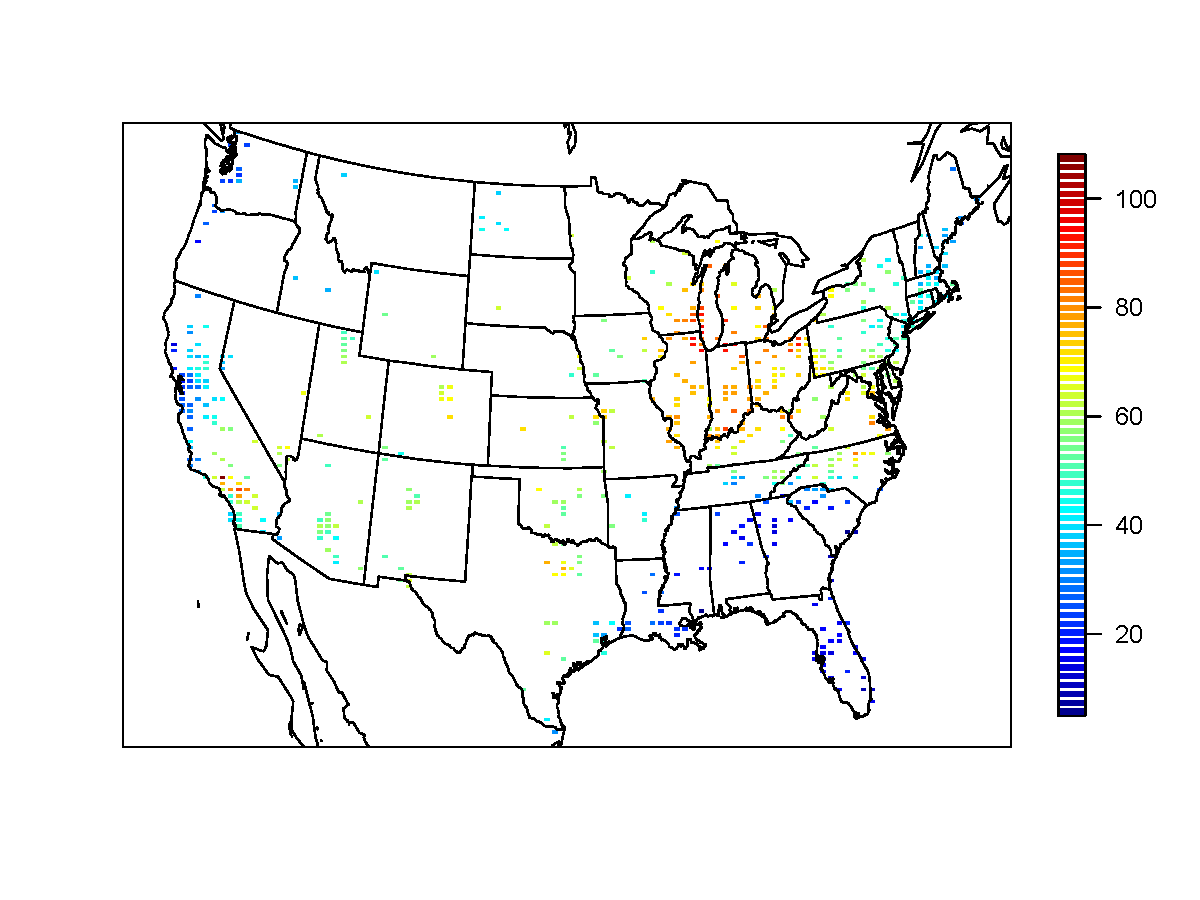
\includegraphics[width=0.8\linewidth, trim={0, 3em, 0, 0}]{plots/ozone-10jul-us}

  Ozone measurements on July 10, 2005, at 1,089 stations across the US
 \end{center}
\end{frame}




% \begin{frame}\frametitle{Low-rank positive-stable representation}
%   \bit\setlength\itemsep{\fill}
%      \item $Z_t$ is max-stable marginally over the random effects $A_{tl}$
%      \item The joint is GEV - asymmetric Laplace
%      \item Dependence is measured by the extremal coefficient $\vartheta$, defined via $$\mbox{Prob}[Z_t(\bs_1)<c, Z_t(\bs_2)<c] = \mbox{Prob}[Z_t(\bs_1)<c]^{\vartheta(\bs_1,\bs_2)}$$
%       \item For the low-rank PS model $$\vartheta(\bs_1,\bs_2) = \sum_{l=1}^L\left[B_l(\bs_1)^{1/\alpha}+B_l(\bs_2)^{1/\alpha}\right]^{\alpha}\in[1,2] $$
%   \eit
% \end{frame}




% \begin{frame}\frametitle{Estimating the EBFs, $B_l(\bs)$}
%   \begin{enumerate}\setlength\itemsep{\fill}
%     \item Use a rank transformation to standardize data for each $\bs$
%     \item Estimate the extremal dependence between each pair of sites (using $\chi$ or madogram), ${\hat \vartheta}(\bs_i,\bs_j)$
%     \item Spatially (4D) smooth the sample dependence measures
%     \item Constrained least squares (next slide) to minimize the distance between sample (${\hat \vartheta}$) and model ($\vartheta$ as a function of the $B$) spatial dependence
%     \item Order the terms by $v_l = \sum_{\bs}B_l(\bs)$
%   \end{enumerate}
% \end{frame}


% \begin{frame}\frametitle{Estimating the EBFs, $B_l(\bs)$}
%   \begin{itemize}\setlength\itemsep{\fill}
%     \item The objective function to estimate the $B_l$ is
%     $$ \sum_{i<j}\left[\hat{\vartheta}(\bs_i,\bs_j) - \vartheta(\bs_i,\bs_j)\right]^2$$
%     where $\vartheta(\bs_i,\bs_j)$ is a function of $B_l$
%     \item The EBFs must satisfy $B_l(\bs)>0$ and $\sum_{l}B_l(\bs)=1$ for all $\bs$
%     \item The solution is approximated by cycling through the sites and solving a series of constrained optimization problems
%   \end{itemize}
% \end{frame}



% \begin{frame}\frametitle{Contrasts with PCA}
%   \bit\setlength\itemsep{\fill}
%   \item Basis functions are not orthonormal
%   \item Loadings are positive stable, not Gaussian
%   \item Loadings $A_{lt}$ may not be independent
%   \item Computing $A$ and $B$ is not as simple as a few matrix operations
%   \eit
% \end{frame}

% \begin{frame}\frametitle{Analogy with PCA}
%   \bit\setlength\itemsep{\fill}
%   \item Reduces the dimension from $n$ to $L$
%   \item Maps of $B_l(\bs)$ tell us about the most important spatial patterns
%   \item Captures a non-stationary spatial dependence structure
%   \item The $v_l$ tell us how many important features are present
%   \item Loadings $A_{lt}$ can be estimated and fed into future analyses
%   \eit
% \end{frame}


% \begin{frame}\frametitle{Bayesian implementation}
%   \bit\setlength\itemsep{\fill}
%   \item Given the basis function $B_l(\bs)$ we can proceed with\\ MCMC to estimate the remaining parameters
%   \item GEV location:  $\mu_t(\bs) = \beta_{\mu,int}(\bs) + \beta_{\mu,time}(\bs)t$
%   \item GEV scale:  $\log[\sigma_t(\bs)] = \beta_{\sigma,int}(\bs) + \beta_{\sigma,time}(\bs)t$
%   \item GEV shape: $\xi$ for all $\bs$ and $t$
%   \item The $\beta$ have Gaussian process priors
%   \item We use cross-validation (quantile and Bries scores) to select $L$
%   \item Alternative: select $L$ so that $\sum_{l=1}^Lv_l = 0.8$
%   \eit
% \end{frame}


% \begin{frame}\frametitle{Application 1 - forest fires in GA}
%   \bit\setlength\itemsep{\fill}
%   \item The data are the number of acres burned by forest fires each year (1965-2014) in each county of Georgia
%   \item We censor the data at the local 95$^{th}$ percentile, $T(\bs)$
%   \item The censored data are modeled as GEV with spatially-varying location and scale
%   \item The objectives are to map fire risk and determine if it is changing with time
%   \eit
% \end{frame}


% \begin{frame}\frametitle{GA Fires -- time series for each county }
%  \begin{center}
%   \includegraphics[width=1.0\textwidth]{Pic/fire-spag-rand-25}
%  \end{center}
% \end{frame}


% \begin{frame}\frametitle{GA Fires -- picking the threshold}
%  \begin{center}
%   \includegraphics[width=1\textwidth]{Pic/fire-mrl-plots}
%  \end{center}
% \end{frame}

% \begin{frame}\frametitle{GA Fires -- 95th percentile by county, $T(\bs)$}
% \vspace{-40pt}
% \begin{center}
%   \includegraphics[height=1.2\textheight]{Pic/fire-spatial-q95}
%  \end{center}
% \end{frame}

% \begin{frame}\frametitle{Model comparisons}
% \begin{center}
%   {\Large \begin{tabular}{l|cc}
%       $L$ & Brier Score & Quantile score\\ \hline
%       5   & 5.64 & 135.7 \\
%       10  & 5.33 & 127.3 \\
%       15  & 5.00 & 128.3 \\
%       20  & 4.93 & 122.4 \\
%       {\bf 25}  & {\bf 4.78} & {\bf 116.9} \\
%       40  & 4.72 & 115.7
%   \end{tabular}}
%   \end{center}
% \end{frame}


% \begin{frame}\frametitle{GA Fires -- EBF weights, $v_l$}
%   \begin{center}
%     \includegraphics[height=0.9\textheight]{Pic/firev}
%   \end{center}
% \end{frame}

% \begin{frame}\frametitle{GA Fires -- EBF's $B_l(\bs)$}
% \vspace{22pt}
% \begin{center}
%   \includegraphics[width=0.99\textwidth]{Pic/ga-ebf-panel}
% \end{center}
% \end{frame}

% \begin{frame}\frametitle{GA Fires -- Ecoregions}
%   \begin{center}
%     \includegraphics[height=0.9\textheight]{Pic/ga_eco_regions}
%   \end{center}
% \end{frame}





% \begin{frame}\frametitle{Time trend ($\beta_{\mu,time}$, $\beta_{\sigma,time}$) -- posterior mean}
%  \begin{center}
%   \includegraphics[width=1.1\textwidth]{Pic/fire_post_mean}
%  \end{center}
% \end{frame}


% \begin{frame}\frametitle{Time trend ($\beta_{\mu,time}$, $\beta_{\sigma,time}$) -- posterior SD}
%   \begin{center}
%     \includegraphics[width=1.1\textwidth]{Pic/fire_post_sd}
%   \end{center}
% \end{frame}



% \begin{frame}\frametitle{Time trend ($\beta_{\mu,time}$, $\beta_{\sigma,time}$) -- prob $>$ 0}
%   \begin{center}
%     \includegraphics[width=1.1\textwidth]{Pic/fire_post_pos}
%   \end{center}
% \end{frame}



% \begin{frame}\frametitle{Application 2 -- NARCCAP climate model output}
%   \bit\setlength\itemsep{\fill}
%   \item Data consist of annual maximum precipitation at \\697 grid cells in the Eastern US
%   \item The model is run separately for 1969-2000 and 2039-2077
%   \item The objective is the compare the extremes in the two climate periods
%   \item We fit the same model as for the fire data except without censoring
%   \item We fit the model separately for the two periods
%   \eit
% \end{frame}


% \begin{frame}\frametitle{Climate model output for 1969}
%  \begin{center}
%   \includegraphics[height=0.99\textheight]{Pic/1969}
%  \end{center}
% \end{frame}




% \begin{frame}\frametitle{Precip -- EBF weights, $v_l$}
%   \begin{center}
%     \includegraphics[height=0.9\textheight]{Pic/precipv}
%   \end{center}
% \end{frame}

% \begin{frame}\frametitle{Precip -- EBFs $B_l(\bs)$}
% \vspace{22pt}
%  \begin{center}
%   \includegraphics[width=0.99\textwidth]{Pic/precip-ebf-panel}
%  \end{center}
% \end{frame}

\begin{frame}\frametitle{Back to a Gaussian process model}
  \bit\setlength\itemsep{\fill}
  \item The max-stable process is an elegant approach, but does that mean it's the right model?
  \item In reality, it is only an approximation
  \item There are less complicated approximations
  \item For example, we could model daily data as a Gaussian process (GP)
  \item If the goal is spatial interpolation, perhaps this is competitive
\eit
\end{frame}


\begin{frame}\frametitle{GP - asymptotic independence}
  \bit\setlength\itemsep{\fill}
  \item A GP leads to simple interpretation and computing, but asymptotic independence
  \item If $Y(\bs_1)$ and $Y(\bs_2)$ are bivariate normal then $\chi(\bs_1,\bs_2)=0$, i.e., asymptotic independence
  \item This suggests Kriging will not capture extremes
  \item But so much is known for the Gaussian case: nonstationarity, multivariate, numerical approximations, \ldots
  \item Rather than toss it out, can we patch it up?
  \eit
\end{frame}


\begin{frame}\frametitle{Spatial \skewt process}
  A spatial \skewt process (Azzalini and Capitanio, 2014)  resembles a GP but exhibits asymptotic dependence
 \begin{eqnarray}
 Y_t(\bs) &=& \bX(\bs)^\top\bbeta +\lambda\sigma_t|z_t| + \sigma_tv_t(\bs)\nonumber\\
 z_t &\sim& \mbox{Normal}(0,1)\nonumber\\
\sigma_t^2&\sim& \mbox{InvGamma}(a/2,b/2)\nonumber\\
v_t&\sim& \mbox{Spatial GP}\nonumber
 \end{eqnarray}
  \bit\setlength\itemsep{\fill}
  \item Location: $\bX(\bs)^\top\bbeta$
  \item Scale: $b>0$
  \item Skewness: $\lambda\in{\cal R}$
  \item Degrees of freedom: $a>0$
  \eit
\end{frame}



\begin{frame}\frametitle{Good properties}
  \bit\setlength\itemsep{\fill}
  \item Flexible $t$ marginal distribution with four parameters including the degrees of freedom which allows for heavy tails ($a=1$ gives a Cauchy)
  \item Computation on the order of a GP; the only extra steps are $z_t$ and $\sigma_t$ which have conjugate full conditionals
  \item Asymptotic dependence: $\chi(\bs_1,\bs_2)>0$ for all $\bs_1$ and $\bs_2$
  \eit
\end{frame}

\begin{frame}\frametitle{Bad properties and remedies}
  \bit\setlength\itemsep{1em}
  \item Modeling all the data (bulk and extreme) can lead to poor tail probability estimates if the model is misspecified
  \item Long-range dependence: $\chi(\bs_1,\bs_2)>0$ for all $\bs_1$ and $\bs_2$ even if $\bs_1$ and $\bs_2$ are far apart
  \item This occurs because all sites share $z_t$ and $\sigma_t$
  \item Remedies:
  \bit
    \item We use a censored likelihood to focus on the tails
    \item We propose a local \skewt process
  \eit
  \eit
\end{frame}

\begin{frame}\frametitle{Censored likelihood}
  \bit\setlength\itemsep{\fill}
  \item Censored likelihood: We censor the data
  $${\tilde Y}_t(\bs) =\left\{\begin{array}{ll}
  T & \text{for } Y_t(\bs)\le T\\
  Y_t(\bs) & \text{for } Y_t(\bs)>T
  \end{array}\right.$$
  \item Censoring is handled using standard Bayesian imputation methods
  \item The threshold $T$ is chosen by cross-validation
  \item If $T$ is moderately extreme in the distribution (e.g. $q(0.75)$), set $\lambda = 0$
  \eit
\end{frame}

\begin{frame}\frametitle{Local \skewt process}
  \bit\setlength\itemsep{\fill}
  \item Let the knots $\bv_{t1},...,\bv_{tK}$ follow a homogeneous Poisson process over the domain of interest (in practice we fix $K$)
  \item Associated with each is
  \begin{itemize}
    \item $z_{tk}\sim\mbox{Normal}(0,1)$
    \item $\sigma_{tk}^2\sim\mbox{InvGamma}(a/2,b/2)$
  \end{itemize}
  \item The knots partition the domain if we assign location $\bs$ to subregion $k=\argmin_{l}||\bs-\bv_{tl}||$
  \item If $\bs$ is in subregion $k$ then $$Y_t(\bs) = \bX(\bs)^T\bbeta +\lambda\sigma_{tk}|z_{tk}| + \sigma_{tk}v_t(\bs)\nonumber$$
  \item The marginal distribution remains a $t$, but partitioning breaks long-range spatial dependence
  \eit
\end{frame}

\begin{frame}\frametitle{$\chi$-statistic by $h=||\bs_1-\bs_2||$}
 \begin{center}
  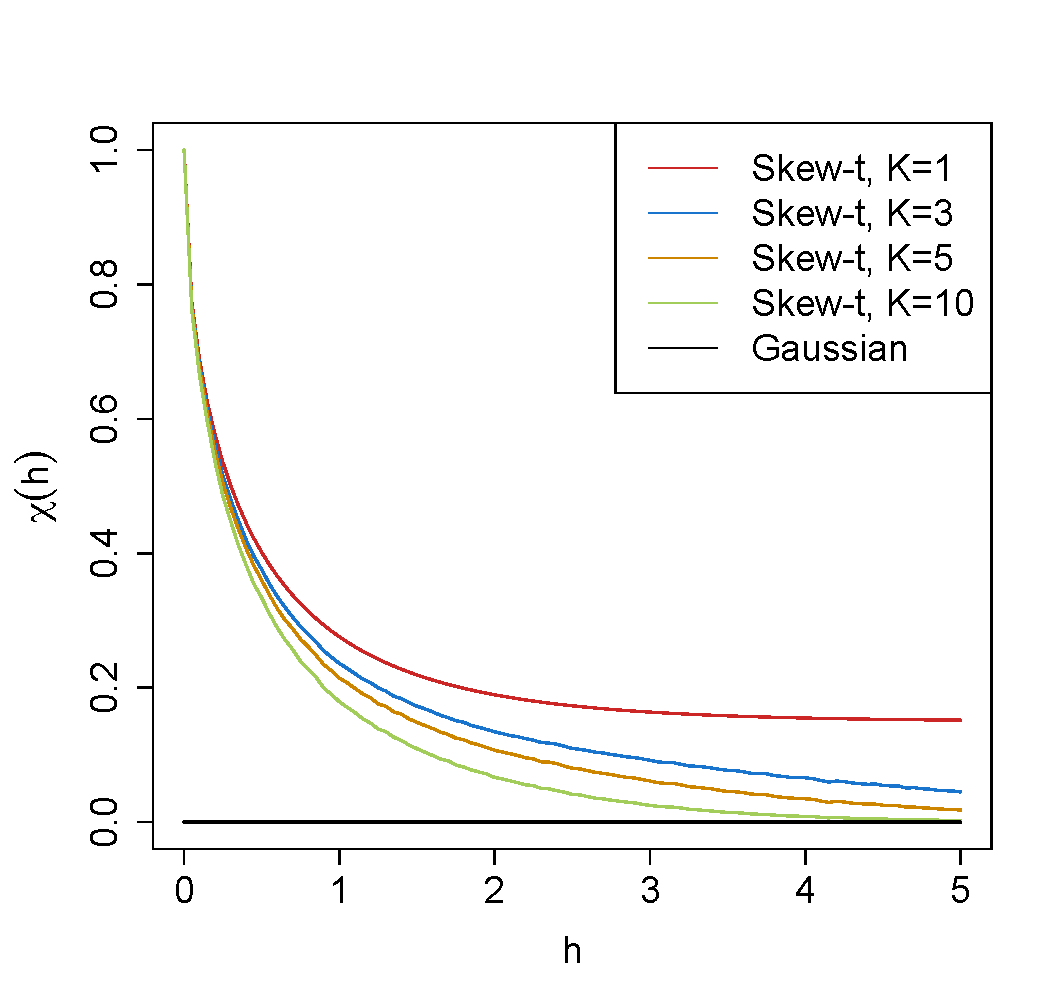
\includegraphics[height=0.8\textheight]{plots/chi-h}
 \end{center}
\end{frame}

\begin{frame}\frametitle{Temporal dependence}
  \bit\setlength\itemsep{1em}
    \item It may not be reasonable to assume that observations are temporally independent (e.g. flooding, high temperatures)
    \item Temporal dependence is handled through the $z_{tk}$, $\sigma_{tk}$ and $\bv_{tl}$
    \item Method:
    \bit\setlength\itemsep{0.5em}
      \item Use a copula to transform parameters to \emph{nice} space (i.e. $\mathcal{R}$)
      \item AR(1) structure imposed on parameters in transformed space
      \item Transform back to original parameter space to preserve \skewt
    \eit
  \eit
\end{frame}


\begin{frame}\frametitle{Results of a simulation study}
  In terms of Brier scores for spatial prediction:\vspace{1em}
  \bit\setlength\itemsep{1em}
  \item Data generated as a GP:
  \bit
    \item \skewt is close to GP
    \item max-stable is 15\% -- 30\% worse than GP
  \eit
  \item Data generated as a \skewt with multiple partitions:
  \bit
    \item \skewt is 15\% better than GP
    \item max-stable is 30\% worse than GP
  \eit
  \item Data generated as asymmetric logistic (max-stable):
  \bit
    \item \skewt is close to GP
    \item max-stable performs 10\% better than GP
  \eit
  \item Data generated as Brown-Resnick (max-stable):
  \bit
    \item \skewt performs 40\% -- 60\% better than GP
    \item max-stable performs 40\% -- 60\% better than GP
  \eit
  \eit
\end{frame}


\begin{frame}\frametitle{Application to ozone}
  \bit\setlength\itemsep{\fill}
  \item The USEPA has an extensive network of ozone monitors throughout the US
  \item We will analyze ozone for 31 days in July, 2005 at $n=1,089$ stations
  \item Currently the EPA regulates the annual 99$^{th}$ percentile
  \item Our objective is to map the probability of an extreme ozone event
  \eit
\end{frame}

\begin{frame}\frametitle{Ozone on July 10}
  \begin{center}
    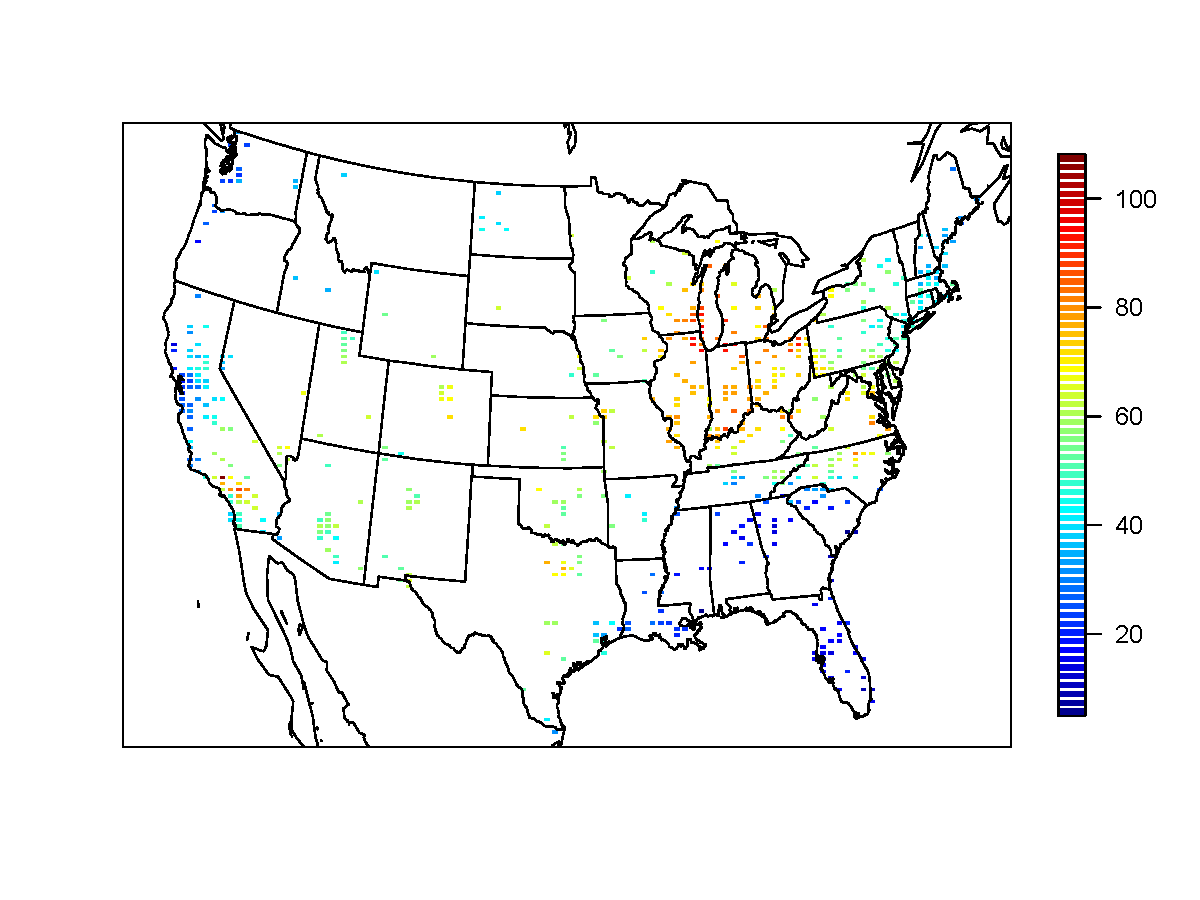
\includegraphics[width=1.2\textheight]{plots/ozone-10jul-us}
  \end{center}
\end{frame}

\begin{frame}\frametitle{Q-Q plots}
  \begin{center}
    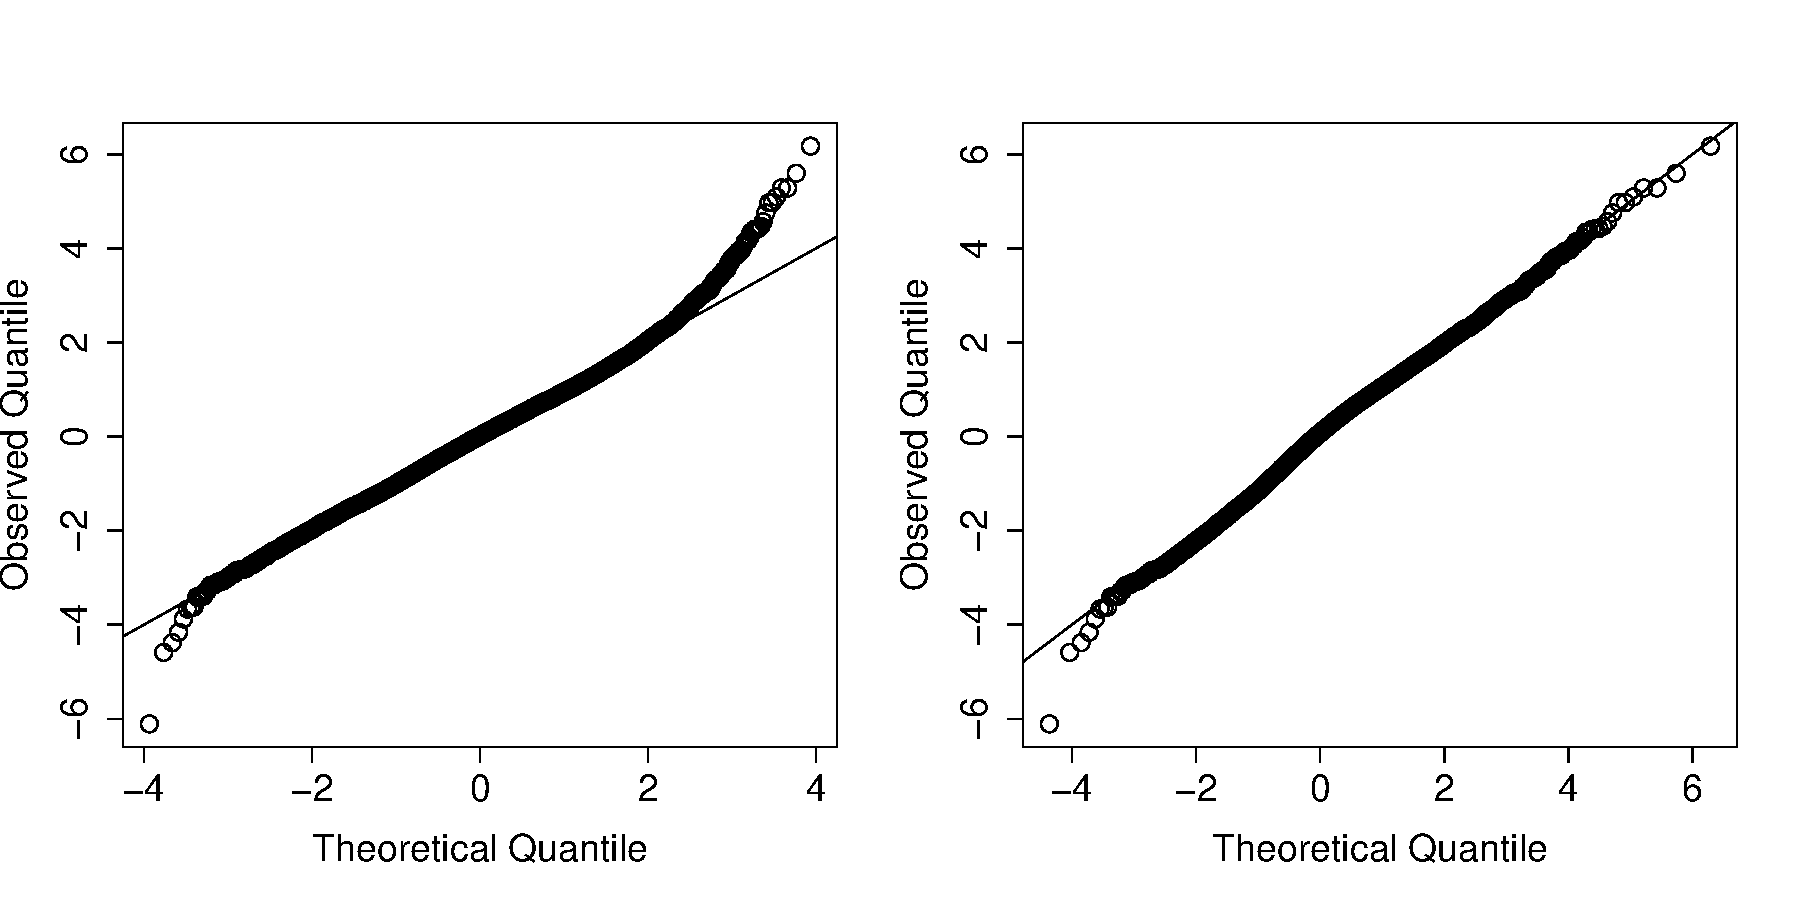
\includegraphics[width=0.9\textheight]{plots/qq-res}

    Gaussian Q-Q plot (left) and skew-$t$ with $a = 10$ and $\lambda = 1$ Q-Q plot (right)
  \end{center}
\end{frame}

\begin{frame}\frametitle{Cross-validation}
  \bit\setlength\itemsep{\fill}
  \item We split the sites into training and testing
  \item We found that $K=15$ knots and censoring at $T$ equal to the median with no time series gave the best results
  \item Results were not sensitive to these tuning parameters
  \item This model was 5\% more accurate (Brier score) than GP
  \item The max-stable model fit was 15\% less accurate than GP
  \eit
\end{frame}

\begin{frame}\frametitle{Fitted 99$^{th}$ percentile - Gaussian}
  \begin{center}
    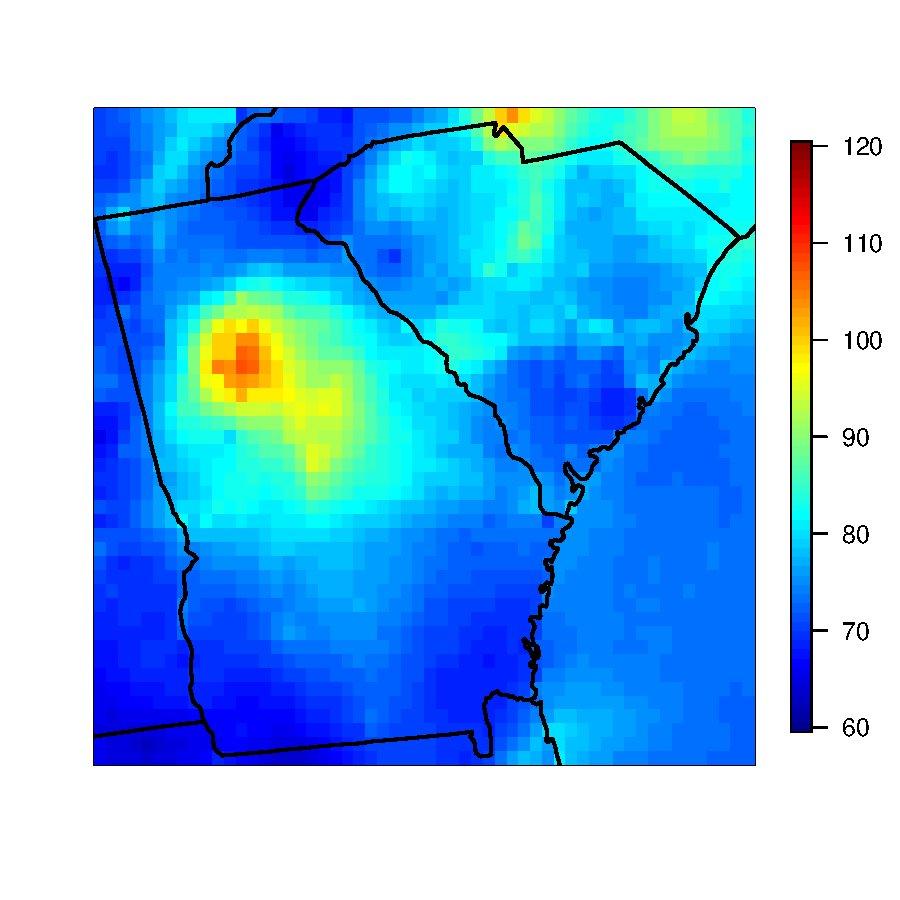
\includegraphics[width=0.45\linewidth]{plots/q99gaus}
    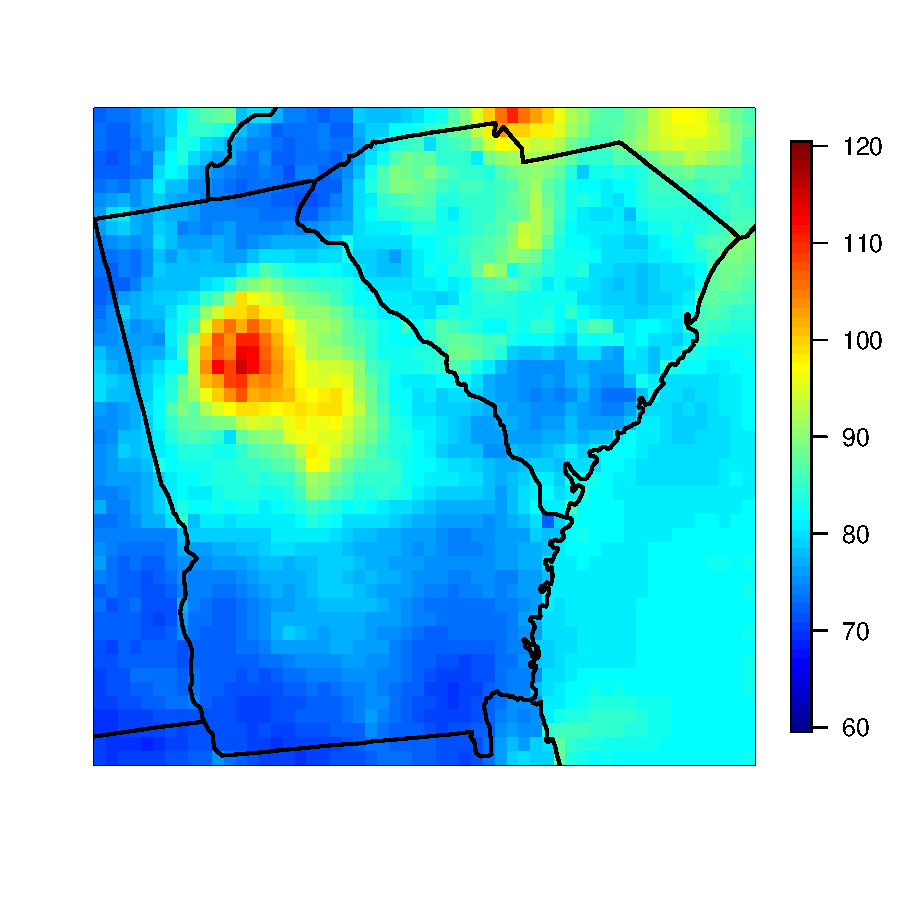
\includegraphics[width=0.45\linewidth]{plots/q99skewtTS}

    Gaussian (left) Symmetric-$t$, 10 knots, T = 75, Time series (right)
  \end{center}
\end{frame}

% \begin{frame}\frametitle{Fitted 99$^{th}$ percentile - Thresholded $t$}
%   \begin{center}



%   \end{center}
% \end{frame}

\begin{frame}\frametitle{Difference (Thresholded $t$ - Gaussian)}
  \begin{center}
    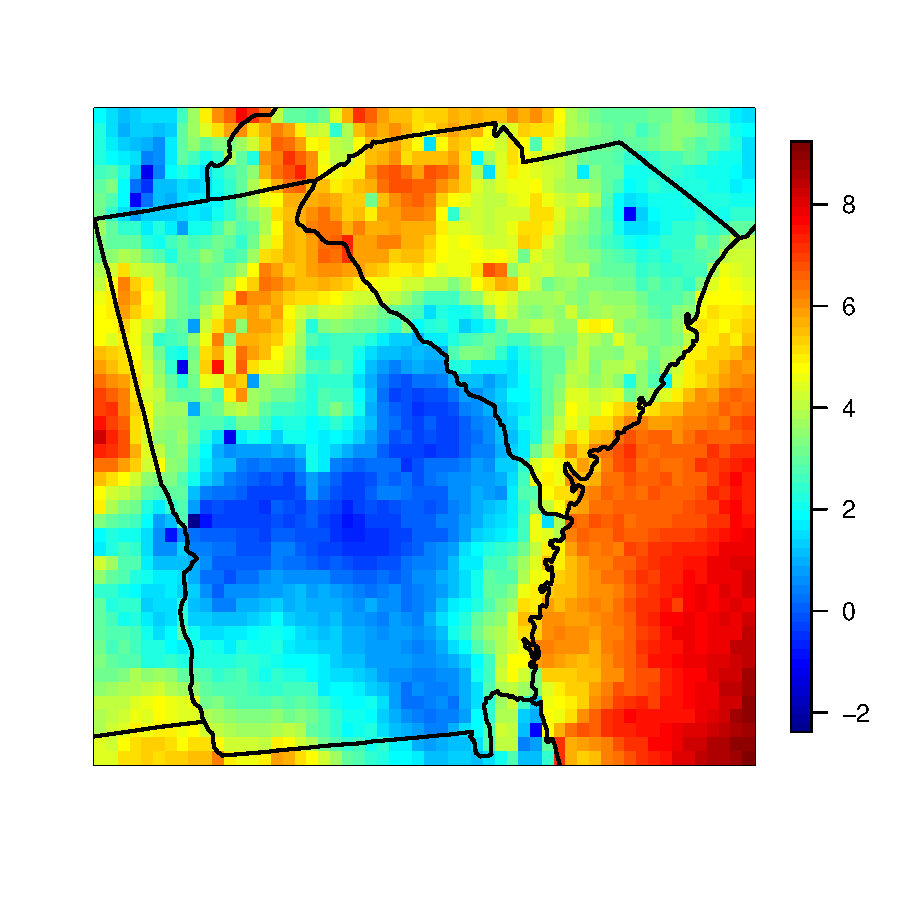
\includegraphics[width=0.55\linewidth]{plots/q99diffgausskewt}

    Difference between Symmetric-$t$, 10 knots, T = 75 and Gaussian
  \end{center}
\end{frame}



\begin{frame}\frametitle{Summary}
  \bit\setlength\itemsep{\fill}
  \item Our proposed method can handle large datasets
  \item The proposed model gives a balance between theoretical properties and computational feasibility
  % \item This should at least be used as a benchmark for more sophisticated approaches
  \item Work supported by NSF, NIH, DOI, and EPA
  \item Thanks!
  \eit
\end{frame}

\end{document}

